Malheureusement,
le \reffact{sep-isolated-zero} échoue dans la tentative de généralisation à $\big( \CC - \frac{\pi}{2} \ZZ \big)^3$ de l'identité
$ \tan \alpha \tan \beta
+ \tan \beta  \tan \gamma
+ \tan \gamma \tan \alpha
= 1$,
celle-ci s'obtenant sans effort comme ci-dessous sous les contraintes géométriques
$(\alpha ; \beta ; \gamma) \in \big( \RRsp \big)^3$
et
$0 < \alpha + \beta + \gamma < \frac{\pi}{2}$.

\begin{center}
	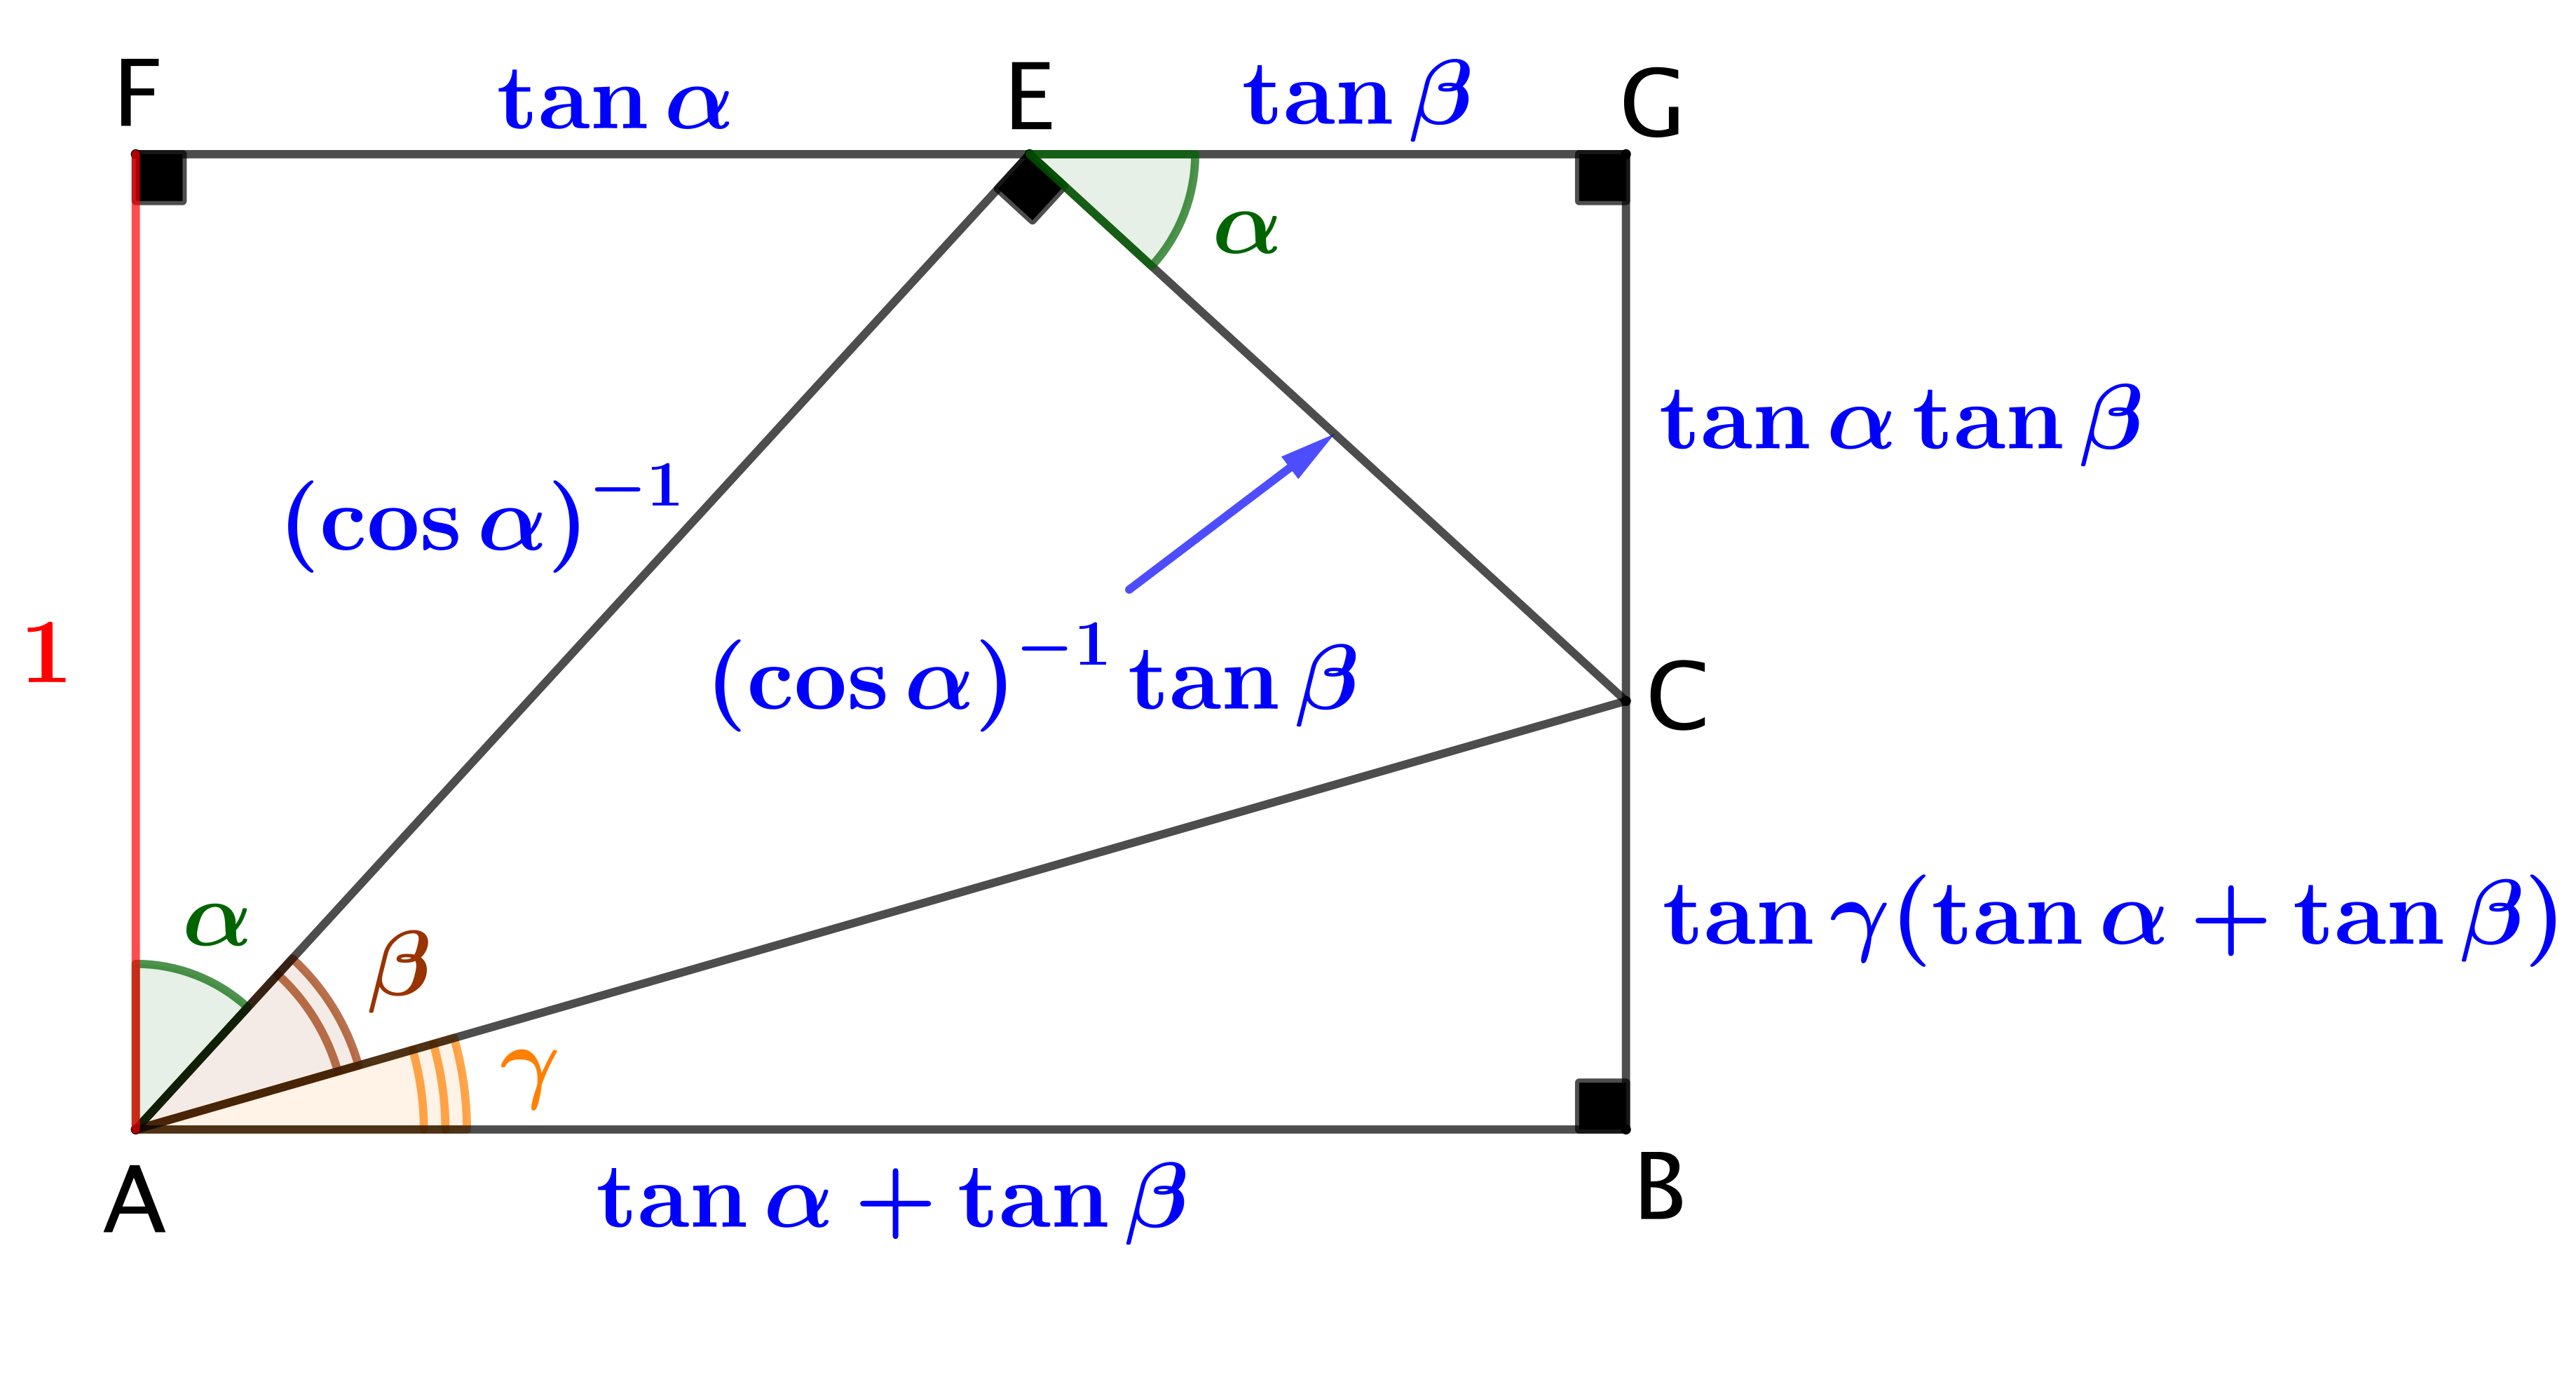
\includegraphics[scale=.75]{sum-tan-prod.png}
\end{center}







\newpage




Que faire si nous avons des formules trigonométriques impliquant deux variables, ou plus?
Par exemple,
pour
$(\alpha ; \beta) \in \big( \RRsp \big)^2$ tel que $0 < \alpha + \beta < \frac{\pi}{2}$,
le dessin suivant nous donne
$\cos(\alpha + \beta) = \cos \alpha \cos \beta - \sin \alpha \sin \beta$
et
$\sin(\alpha + \beta) = \cos \alpha \sin \beta + \sin \alpha \cos \beta$.%
\footnote{
    Cette démonstration est très utile pour un cours pré universitaire.
}

\begin{center}
	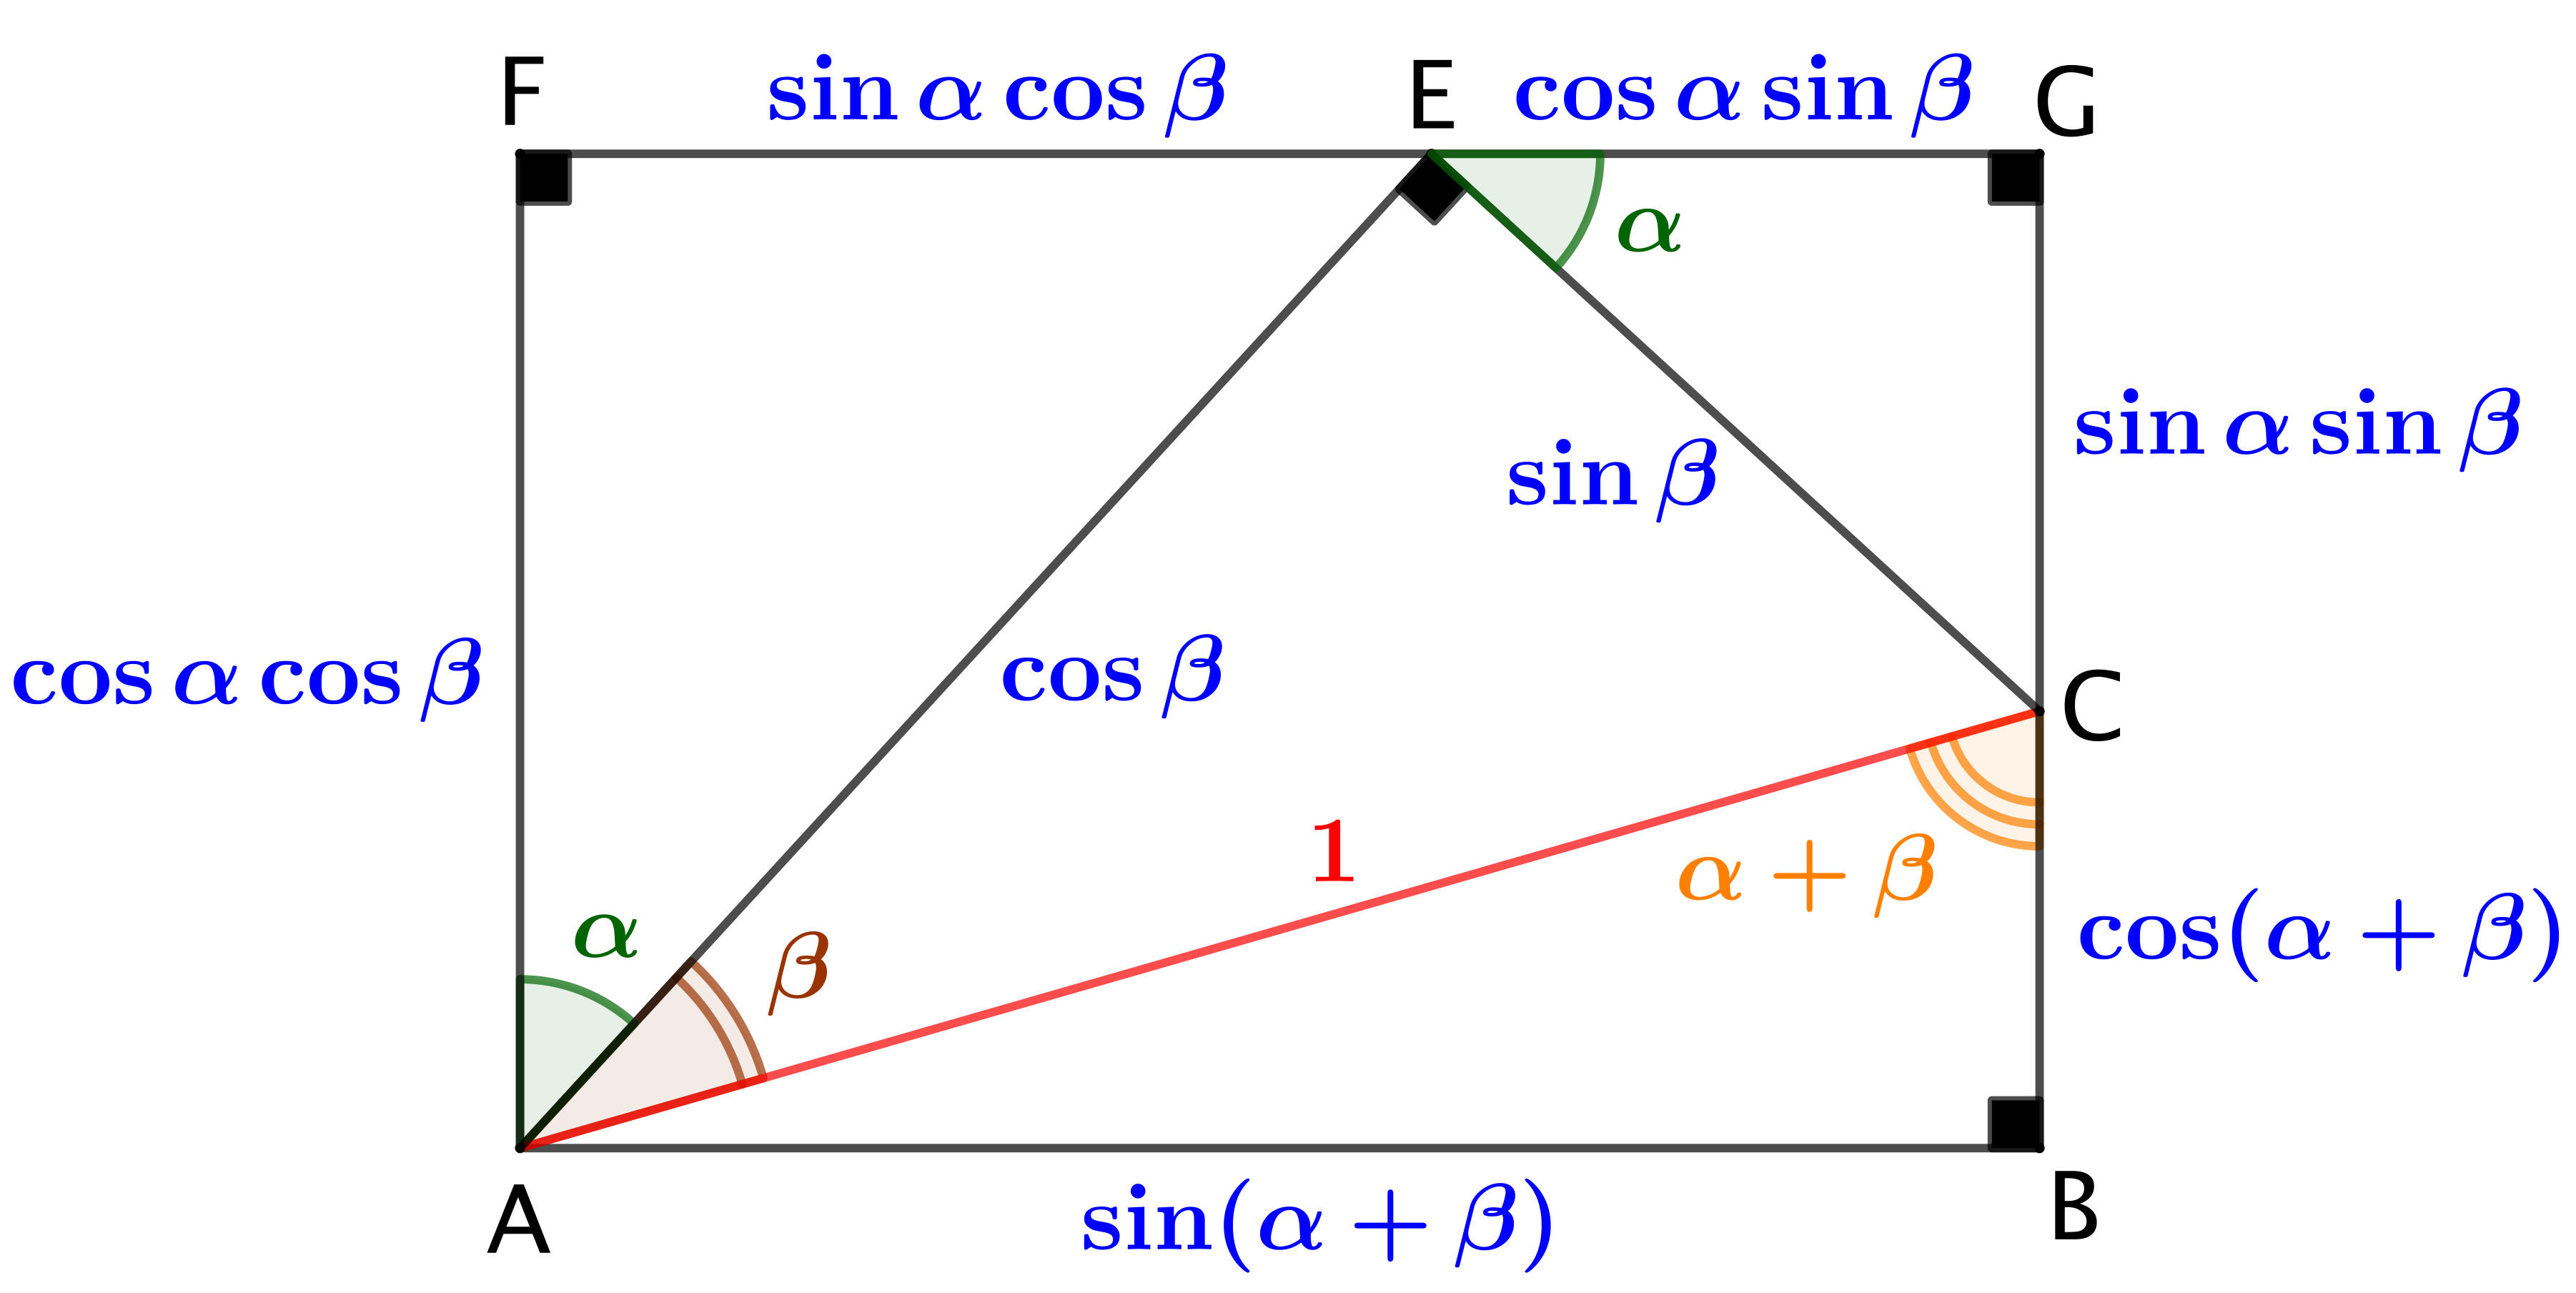
\includegraphics[scale=.7]{add-trigo-formulas.png}
\end{center}

Le fait \ref{multi-isolated-zero} ci-dessous, qui généralise le fait \ref{isolated-zero}, implique la validité des formules trigonométriques précédentes sur $\CC^2$ tout entier en faisant les choix ci-après.%
\footnote{
    L'ouvert d'annulation est l'intérieur d'un triangle.
}
Nous voilà sauvés!
%
\begin{itemize}[label=\small\textbullet]
	\item $f_1(\alpha ; \beta) = \cos(\alpha + \beta) - \cos \alpha \cos \beta + \sin \alpha \sin \beta$

	\item $f_2(\alpha ; \beta) = \sin(\alpha + \beta) - \cos \alpha \sin \beta - \sin \alpha \cos \beta$
\end{itemize}


% ----------- %


\newpage





\begin{defi}
    Soient $n \in \NNs$
    et
    $\Omega$ un sous-ensemble de $\CC^n$.
    %
    Pour $k \in \ZintervalC{1}{n}$,
    la \focus{k\ieme\ projection} de $\Omega$ est l'ensemble $\pi_k(\Omega) = \setgene{\omega \in \CC \mid \exists (z_1 ; ... ; z_{k-1} ; \omega ; z_{k+1} ; ... ; z_n) \in \Omega}$,
    et
    la \focus{k\ieme\ section} de $\Omega$ est l'ensemble $\sigma_{\leq k}(\Omega) = \setgene{(\omega_1 ; ... ; \omega_k) \in \CC^k \mid \exists (\omega_1 ; ... ; \omega_k ; z_{k+1} ; ... ; z_n) \in \Omega}$.
    
\end{defi}



\begin{defi}
    Soient $n \in \NNs$
    et
    $\Omega \subseteq \CC^n$ un ensemble non vide.
    Pour $f: \Omega \rightarrow \CC$
    et
    $k \in \ZintervalC{1}{n}$,
    la \focus{k\ieme\ restriction} de $f$ est définie par
    $f_k: z \in \pi_k(\Omega) \mapsto f(z_1 ; ... ; z_{k-1} ; z ; z_{k+1} ; ... ; z_n) \in \CC$.%
	\footnote{
		Avec des abus de notations évidents.
	}
\end{defi}


\begin{defi}
    Soient $n \in \NNs$
    et
    $\Omega \subseteq \CC^n$ un ouvert non vide.
    Une fonction $f: \Omega \rightarrow \CC$ sera dite \focus{séparablement analytique} sur $\Omega$,
    si $\forall k \in \ZintervalC{1}{n}$,
    la k\ieme\ restriction de $f$ est analytique sur $\pi_k(\Omega)$ (qui est un ouvert non vide de $\CC$).
\end{defi}


\begin{fact} \label{multi-isolated-zero}
    Soient $n \in \NNs$,
    $\Omega \subseteq \CC^n$ un ouvert connexe non vide
    et
    $f: \Omega \rightarrow \CC$ une fonction séparablement analytique.
	Si $f$ s'annule sur un ouvert non vide de $\Omega$,
	alors $f$ s'annule sur $\Omega$ tout entier. 
\end{fact}


\begin{proof}
	Raisonnons par récurrence sur $n \in \NNs$ pour démontrer la validité de la propriété $\setproba{P}(n)$ définie par
	\emph{\og 
		Pour toute fonction séparablement analytique $f: \Omega \rightarrow \CC$ sur un ouvert connexe non vide $\Omega \subseteq \CC^n$,
		si $f$ s'annule sur un ouvert non vide de $\Omega$,
		alors $f$ s'annule sur $\Omega$ tout entier. 
	\fg}\kern2pt.
	%
	\begin{itemize}[label=\small\textbullet]
		\item \textbf{Cas de base.}
		%
		$\setproba{P}(1)$ découle directement du \reffact{isolated-zero}.


		\item \textbf{Hérédité.}
		%
		Supposons $\setproba{P}(n)$ valide pour un naturel $n$ quelconque.
		Soit $f$ une fonction séparablement analytique à $(n + 1)$ variables vérifiant les conditions de la propriété $\setproba{P}(n + 1)$.
		Notons $V \subseteq \Omega$ l'ouvert non vide sur lequel $f$ est nulle.
		%
		Quitte à réduire $V$, on peut supposer que
		$V = \dprod_{k=1}^{n+1} \CdiscO{\alpha_k}{r}$
		avec $r > 0$ et les $\alpha_k$ des complexes fixés.
		%
		\begin{enumerate}
		    \item Pour $\omega \in \CdiscO{\alpha_{n+1}}{r}$ fixé,
		    posons
		    $f_\omega: (z_1 ; ... ; z_n) \in \sigma_{\leq n}(\Omega) \mapsto f(z_1 ; ... ; z_n ; \omega) \in \CC$.
		    Comme $f_\omega$ vérifie les conditions de la propriété $\setproba{P}(n)$, par hypothèse de récurrence,
		    $f_\omega(z_1 ; ... ; z_n) = 0$, 
		    soit $f(z_1 ; ... ; z_n ; \omega) = 0$,
		    pour $(z_1 ; ... ; z_n) \in \sigma_{\leq n}(\Omega)$.


		    \item Pour $z_1$ , ... , $z_n$ des complexes quelconques de $\sigma_{\leq n}(\Omega)$,
		    posons $\ell(z) = f(z_1 ; ... ; z_n ; z)$.
		    Le point précédent montre que $\ell$ vérifie $\setproba{P}(1)$,
		    donc, d'après le cas de base,
		    $\ell(z) = 0$,
		    soit $f(z_1 ; ... ; z_n ; z) = 0$,
		    pour tout complexe $z \Omega \cap \prod_{i=1}^n {z_k} \times {\omega}$.


		    \item Finalement, $f(z_1 ; ... ; z_n ; z) = 0$ pour tous complexes $z_1$ , ... , $z_n$ et $z$.
		    Autrement dit, nous avons déduit la validité de $\setproba{P}(n+1)$ à partir de celle de $\setproba{P}(n)$.
		\end{enumerate}
		
		
		\item \textbf{Conclusion.}
		%
		Par récurrence sur $n \in \NNs$, la propriété $\setproba{P}(n)$ est vraie pour tout naturel non nul $n$.
	\end{itemize}

	\null\vspace{-6ex}
\end{proof}

















